\documentclass[relatorio,oneside]{iagtese}	       % subclasse relatorio do iagtese
										%
%\documentclass[relatorio,oneside]{iagtese_en}	% subclasse relatorio do iagtese
										% em ingles. Para escrever o 
										% relatorio em ingles, descomente
 										% esta linha e comente a linha
                                            					% anterior.
\def\today{Mar�o de 2010 a Agosto de \number\year}% per�odo a que se refere o relat�rio
										%
										%	
\begin{document}							% in�cio do documento
										% 				
\institution{Universidade de S�o Paulo \\ Instituto de Astronomia, Geof�sica e Ci�ncias Atmosf�ricas \\ Departamento de Astronomia}

\title{T�tulo do trabalho}

\translator{{Tese/Disserta��o apresentada ao Departamento de Astronomia do Instituto de Astronomia, Geof�sica e Ci�ncias Atmosf�ricas da Universidade de S�o Paulo como requisito parcial para a obten��o do t�tulo de Mestre/{}Doutor em Ci�ncias.\\ \\
�rea de Concentra��o: Astronomia\\
Orientador(a): Prof.($^{\rm a}$) Dr.($^{\rm a}$) Orientador(a)}}

\author{Autor}

\date{S�o Paulo \ano}
							% arquivo para inserir a capa
										% 
\titulo									% 
										%
\assinatura								% folha com assinaturas								
										%
\chapter{Cap�tulo 01}
\label{cap01}

\section{como incluir cita��es utilizando bibTeX}

\begin{verbatim}O comando \citet{doutorado} produz:\end{verbatim}
\citet{doutorado}

\begin{verbatim}O comando \citet{mestrado} produz:\end{verbatim}
\citet{mestrado}

\begin{verbatim}O comando \citet*{artigo1} produz:\end{verbatim}
\citet*{artigo1}

\begin{verbatim}O comando \citet{artigo2} produz:\end{verbatim}
\citet{artigo2}

\begin{verbatim}O comando \citet{bethe} produz:\end{verbatim}
\citet{bethe}

\begin{verbatim}O comando \citet{livro} produz:\end{verbatim}
\citet{livro}

\begin{verbatim}O comando \citet{feynman} produz:\end{verbatim}
\citet{feynman}

\begin{verbatim}O comando \cite{salpeter} produz:\end{verbatim}
\cite{salpeter}

\section{pr�xima se��o}

\subsection{subse��o}

\subsubsection{subsubse��o}

\paragraph{par�grafo}
  	  					% inserir os cap�tulos do seu 							
										% trabalho
\chapter{Cap�tulo 02}
\label{cap02}

Base de dados. Citar figura \ref{identificador}.

\begin{figure}[!ht]
\begin{center}
\setcaptionmargin{1cm}
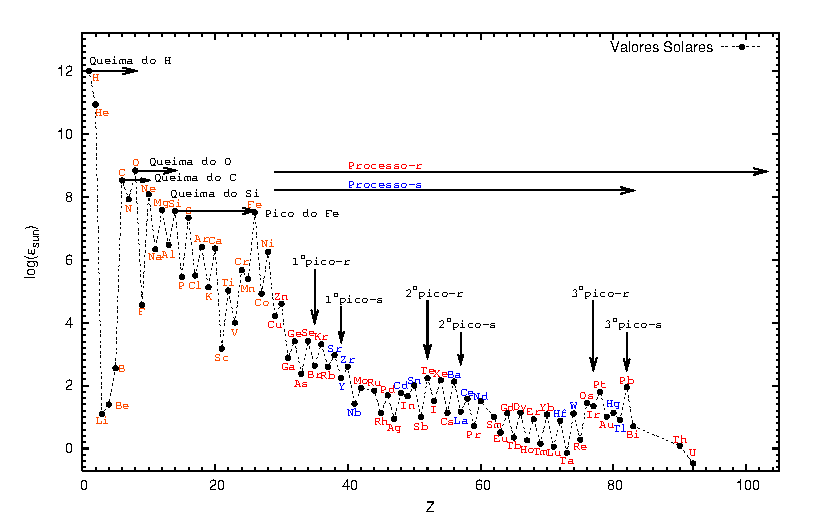
\includegraphics[width=1.0 \columnwidth,angle=0]{fig/solar_grevesse.eps}
\caption{Legenda da figura.} 
\label{identificador}
\end{center}
\end{figure}


\begin{center}
\setcaptionmargin{1cm}
\scriptsize
\begin{longtable}{lcccc}
\caption[Resumo da legenda da tabela (aparece na lista de figuras)]{Exemplo de tabela feita com o longtable.}\\
\hline \hline \\[-2ex]
\multicolumn{1}{c}{Coluna1} &
\multicolumn{1}{c}{Coluna2} &
\multicolumn{1}{c}{Coluna3} &
\multicolumn{1}{c}{Coluna4} &
\multicolumn{1}{c}{Coluna5} 

\\[0.5ex] \hline
\\[-1.8ex]

\endfirsthead

\multicolumn{5}{c}{\footnotesize{{\slshape{{\tablename} \thetable{}}} - Continua��o}}\\[0.5ex]

\hline \hline\\[-2ex]

\multicolumn{1}{c}{Coluna1} &
\multicolumn{1}{c}{Coluna2} &
\multicolumn{1}{c}{Coluna3} &
\multicolumn{1}{c}{Coluna4} &
\multicolumn{1}{c}{Coluna5} 

\\[0.5ex] \hline
\\[-1.8ex]

\endhead

\multicolumn{3}{l}{{\footnotesize{Continua na pr�xima p�gina\ldots}}}\\
\endfoot
\hline

\endlastfoot

1 & 2 & 3 & 4 & 5 \\
6 & 7 & 8 & 9 & 10\\

\label{tabela_com_longtable}
\end{longtable}
\end{center}


  	      					% 
										%
\bibliography{tex/bibliografia}					% referencias com bibTeX
										%
										%
\end{document}								% fim do documento
